\documentclass[12pt, a4paper]{extarticle}
\usepackage{cmap}
\usepackage{amsfonts}
\usepackage[T2A]{fontenc}
\usepackage[utf8]{inputenc}
%\usepackage{mathtext}  
\usepackage{amsmath, amsfonts, amssymb}
\usepackage[russian]{babel}
\usepackage[body={17.5cm, 23.5cm},left=3cm, top=2cm, right=2cm]{geometry}
\usepackage{graphicx}
\usepackage{blindtext}
\usepackage{fancyhdr}
\usepackage{graphicx}
\usepackage{ragged2e}
\usepackage{epigraph}
\usepackage{misccorr}  
\usepackage{indentfirst} 
\usepackage{amsmath}
\usepackage{tabularx} 

\usepackage{fancyhdr} 
\usepackage{color}

\usepackage{makecell}
\usepackage{slashbox}

%\parindent{1.25cm} 
\graphicspath{images/}
\setcounter{tocdepth}{6}
\newcommand{\eps}{\varepsilon}
\newcommand{\re}{\operatorname{Re}}
\newcommand{\im}{\operatorname{Im}}
\DeclareMathOperator{\sgn}{sgn}
\renewcommand{\labelitemi}{$-$}
\renewenvironment{itemize}[1][{---\hfil}]{\begin{list}{#1}{\topsep=0pt\parsep=0pt plus 1pt\itemsep=\parsep\leftmargin=0pt \itemindent=\parindent}\addtolength{\itemindent}{\labelwidth}}{\end{list}}

\numberwithin{equation}{section} 

\newtheorem{attachment}{\hspace{12cm}  Приложение}
\renewcommand{\theattachment}{\Alph{attachment}}
%\renewcommand{\newtheorem}{\Alph{attachment}}
%\newtheorem{Conjecture}{Conjecture}[section]

\usepackage{tocloft}
\renewcommand{\cftsecleader}{\cftdotfill{\cftdotsep}}

\begin{document}
\thispagestyle{empty} 
\medskip 

\begin{center} 
	\textbf{МИНОБРНАУКИ РОССИИ\\ 
		\vspace{0.5cm} 
		Федеральное государственное бюджетное образовательное\\ 
		учреждение высшего образования\\ 
		«Ярославский государственный университет им. П.Г. Демидова»}\\ 
	\vspace{0.5cm} 
	{Кафедра математического моделирования}\\ 
	\vspace{1.5cm} 
	
\end{center}
\begin{flushright} 
	Сдано на кафедру\\
	« 
	\underline{\phantom{aaa}} 
	» 
	\underline{\phantom{aaaaaaaaaaaaa}} 2019 г.\\ 
	Заведующий кафедрой\\
	\underline{\phantom{aaa}д. ф.-м. н., профессор\phantom{aaa}}\\ 
	\vspace{0.1cm} 
	\underline{\phantom{aaaaaaaaaaaaa}} С.А. Кащенко
\end{flushright}
\vspace{3cm} 
\begin{center} 
	Курсовая работа\\ 
	\vspace{0.5cm} 
	\textbf{Математическое моделирование движения транспортных потоков}\\ 
	\small{(Направление подготовки магистров 01.04.02 Прикладная математика и информатика)}
	\vspace{3cm} 
\end{center} 

\begin{flushright} 
	Научный руководитель\\ 
	\underline{\phantom{aaa}д. ф-м. н., доцент\phantom{aaa}}\\ 
	\vspace{0.1cm} 
	\underline{\phantom{aaaaaaaaaaaaa}} И.С. Кащенко\\ 
	« 
	\underline{\phantom{aaa}} 
	» 
	\underline{\phantom{aaaaaaaaaaaaa}} 2019 г.\\ 
	\vspace{0.5cm} 
	Студент группы \underline{\phantom{a}ПМИ-11МО\phantom{a}}\\ 
	\vspace{0.1cm} 
	\underline{\phantom{aaaaaaaaaaaaa}} М.А. Погребняк\\ 
	« 
	\underline{\phantom{aaa}} 
	» 
	\underline{\phantom{aaaaaaaaaaaaaa}}2019 г.\\ 
	\vspace{1cm} 
\end{flushright} 
\begin{center} 
	Ярославль 2019 г.
	\vspace{-1cm}  
\end{center} 


\justify 
\setlength{\parindent}{1.25cm} 
\newpage 
\thispagestyle{empty} 
\setcounter{page}{2} 
%\section*{Реферат}
%\vspace{\baselineskip}	

\newpage

\setcounter{page}{2}

%\thispagestyle{empty} 
\tableofcontents 
\newpage 

\section*{Введение}
\addcontentsline{toc}{section}{Введение}
\epigraph{\textit{Рано или поздно всякая правильная математическая идея находит применение в тои или ином деле.}}
{А. Н. Крылов}
В современном мире, где технологии и прогресс с огромной скоростью шагают вперёд, трудно представить, как человек смог бы обходится без мощного инструмента познания окружающей действительности под названием «математическое моделирование». С момента появления человека на земле математическое моделирование стало неотъемлемой частью его жизни. Необходимость в исследовании математических моделей прежде всего влияет на саму жизнь человека. Оно возникает, когда сами объекты или явления недоступны для изучения ввиду опасности, которую они представляют, удалены во времени и в пространстве или исследования связанны с большими материальными потерями и непредвиденными последствиями. Так или иначе математическое моделирование имеет огромную важность в жизни человека и никогда не потеряет свою актуальность.

В настоящее время, в связи с развитием компьютерной техники и постоянным совершенствованием программного обеспечения, математическое моделирование развивается быстрыми темпами. Возрастающие потребности в различных сферах общества, например, разработка и управление техническими устройствами, анализ экономических и социальных процессов, способствуют этому. Все естественные и общественные науки, использующие математический аппарат, по сути занимаются математическим моделированием: заменяют реальный объект его аналогом, отражающим в математической форме важнейшие его свойства, а затем изучают его.  Результаты таких исследований очень содержательны и применимы в повседневной жизни. Математическая модель выражает существенные черты объекта или процесса языком уравнений и других математических средств. 

Метод математического моделирования занимает одно из ведущих мест в исследованиях сложных явлений и процессов, так как позволяет количественно и качественно описать наиболее существенные связи между переменными в системе и применить достаточно развитый математический аппарат и программные средства для анализа явлений, а также для их прогнозирования и управления этими процессами. 

Математическое моделирование очень часто встречается в физике, ведь не зря математику называют языком физики. Эти науки всегда тесно связаны и взаимно обогащают друг друга идеями и методами. Хотя физика и считается наукой о природе, изучающая простейшие и вместе с тем наиболее общие свойства материального мира, но она базируется на моделях объектов материального мира. Поэтому метод математического моделирования изначально зародился в физике, точнее, в математической физике, а затем постепенно начал проникать и в другие науки, где со временем стал очень востребован. Раньше из обширного математического аппарата физики применяли в основном аналитические и полуаналитические методы и приёмы Сейчас все чаще обращаются к математическому моделированию, когда исследуемый физический процесс описывается некоторой математической моделью, представляющей собой систему дифференциальных или интегро-дифференциальных уравнений математической физики. Изучая какие-либо физические явления, исследователь прежде всего создаёт его математическую идеализацию или, другими словами, математическую модель, то есть, пренебрегая второстепенными характеристиками явления, он записывает основные законы, управляющие этим явлением, в математической форме и очень часто эти законы выражаются в виде дифференциальных уравнений. Для составления математической модели в виде дифференциальных уравнений нужно, как правило, знать только локальные связи и не нужна информация обо всем физическом явлении в целом.

Современные компьютерные технологии позволили подойти к решению проблемы математического моделирования транспортных потоков. Основы математического моделирования, закономерностей дорожного движения были заложены в 1912 году русским учёным, профессором Г.Д. Дубелиром. В своей книге «Городские улицы и мостовые» \cite{Street} он положил начало развитию такой отрасли как моделирование транспортных потоков. За прошедший век непрерывных исследований выработалось много хороших моделей, которые помогают сегодня строить качественные и быстрые дороги и регулировать транспортные потоки. Но проблема транспортных потоков никуда не уходит, а на оборот только возрастает в связи с увеличением численности людей на земле, строительством и расширением городов и сообщений между ними и как следствие развитием и модернизацией транспорта.  Транспорт— одна из ключевых систем городского организма, которую по важности уместно сравнить с кровоснабжением. Именно транспорт позволяет городу в полной мере выполнять связующую, коммуникационную и обеспечивающую функции. Тема транспорта касается практически каждого городского жителя, и тем важнее становятся усилия по систематизации управления дорожным движением на транспортной сети городов, ведь без грамотно проработанной транспортной модели, управлять городскими потоками практически, невозможно. Например, в определённом месте городской магистрали систематически возникают автомобильные пробки. Если модель транспортной системы отсутствует, высока вероятность принятия ошибочного решения, результатом которого станет перенос пробки на новое место или создание новых автомобильных пробок. Создавая подобные модели, можно планировать транспортные системы современных городов. Изменения в одной части такой системы приводят к появлению изменений в других ее частях. Насколько увеличится автомобильный поток, если сделать дорогу более широкой? Почему автомобильная пробка регулярно образуется на конкретном перекрёстке? Какой потенциал создаст развитие системы городского общественного транспорта для изменения застройки в черте города? Что случится, если внести изменения в режим работы определённого светофора? Ответить на все эти, а также многие другие вопросы позволяет моделирование транспортной системы. Одна из наиболее трудных проблем, стоящих перед исследователем
организации движения — это превращение реальной дорожно-транспортной обстановки, включающей водителей, автомобили, устройства регулирования движения и дорогу, в набор математических символов и зависимостей, воспроизводящих их поведение. Именно тут математическое моделирование является основой, которая позволяет рассматривать подобные взаимодействия в целом. Решение задач моделирования транспортных потоков и внедрение этих технологий позволяет значительно улучшить ситуацию на проезжей части дороги, снизить тенденцию к образованию транспортных пробок, перегрузке или недогрузке отдельных линий и узлов транспортной сети, снижению уровня аварийности, а также помогает решать и экологические проблемы.

\newpage
\section{Постановка задачи} 
Используя теоретические подходы исследования движения транспортных потоков, составить математическую модель для описания движения транспортных потоков. Данная модель должна представлять из себя набор дифференциальных уравнений и иметь практическую значимость. Полученную модель необходимо исследовать, используя компьютерные технологии.   

\newpage
\section{????}
Научное исследование транспортных потоков началось в 1910-х годах прошлого века и продолжает развиваться в наши дни. В условиях стремительного расширения городов и развития их инфраструктуры становится всё более актуальным моделирование потоков автомобильного транспорта. За более чем вековую историю исследований было создано и применено множество различных теорий и методов, а так же было создано множество различных моделей. Всё множество таких моделей можно разделить на три группы, в зависимости от основного подхода, используемого при моделировании.

Первая группа - это \textbf{вероятностные} модели. В этих моделях транспортный поток рассматривается как результат взаимодействия транспортных средств на элементах транспортной сети.
Такой подход используют стохастические модели.

Вторая группа - это \textbf{макроскопические} модели. В таких моделях автомобильная среда рассматривается на трассе как нечто цельное. Обычно её уподобляется какому-либо физическому потоку. Существует целый ряд газокинетических, гидродинамических моделей, использующих такой подход.

Третья группа - это \textbf{микроскопические} модели. В этих моделях каждый автомобиль рассматривается как отдельная частица со своей скоростью и конечной целью. К таким моделям можно отнести модели, основанные на теории клеточных автоматов и модели, основанные на принципе следования за лидером.

В данной работе рассматриваются различные модели, построенные с использованием микроскопических методов, а именно подход, основанный на движении транспортных средств друг за другом {\it(follow the leader)}.

Под \textbf{транспортным потоком} будем понимать {\it количество единиц транспортных средств одного вида транспорта, проследовавших определённый участок пути в течение установленного промежутка времени} \cite{TrafficFlow}. В качестве транспортного средства рассмотрим автомобиль и будем называть его \textbf{лидером}, если за ним есть другой автомобиль, или \textbf{преследователем}, если перед ним есть другой автомобиль. Причём, один и тот же автомобиль может являться одновременно и преследователем для впереди идущего, и лидером для позади идущего (рис. \ref{car_following}). 

\begin{figure}[h!]  
	\begin{center}
		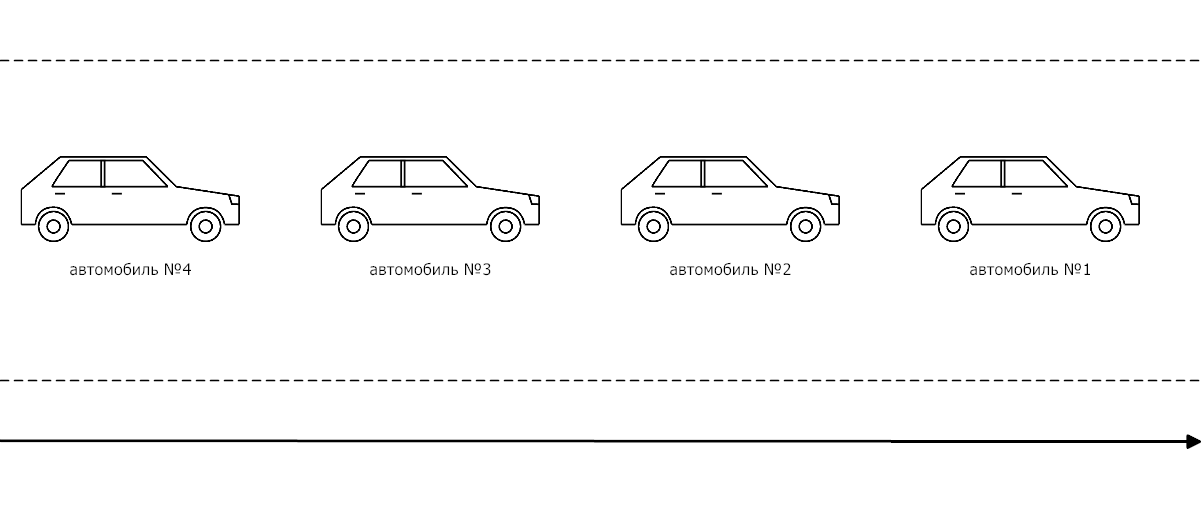
\includegraphics[keepaspectratio,width=160mm,height=70mm]{Images/car_following.png}
	\end{center}
	\caption{Автомобили, следующие друг за другом.}
	\label{car_following}
\end{figure}

Рассмотрим парадигму автомобиля, которая основана на очень простом правиле и уже довольно давно известна в литературе. Так как автомобили следуют друг за другом, преследователь всегда пытается максимизировать свою скорость с двумя ограничениями: ограничением ускорения и ограничением безопасности. Впервые данная парадигма была высказана ещё в 1975 \cite{GippsModel} и математически выглядит следующим образом:

\begin{equation} \label{following_paradigm}
v_f(t) = \min(v_f^d(t), v_f^s(t)),
\end{equation}
где $v_f(t)$ - скорость преследователя в момент времени $t$, $v_f^d(t)$ - максимальная возможная скорость с \textbf{ограничением ускорения} (demand speed), $v_f^s(t)$ - максимальная возможная скорость с \textbf{ограничением безопасности} (supply speed).

Под ограничение ускорения стоит понимать физические ограничения скорости и ускорения транспортного средства, а также условия комфорта, необходимые водителю. Оно описывает траекторию транспортного средства, которое свободно разгоняется до максимальной желаемой скорости при отсутствии впереди идущих транспортных средств. Это не всегда постоянное значение: например, оно может зависеть от скорости автомобиля. Ограничение безопасности - это то, как траектория транспортного средства зависит от впереди идущего транспортного средства (лидера).

\section{Модель свободного движения}

Для начала рассмотрим простую ситуацию, когда на дороге есть всего один автомобиль, для которого нет никаких ограничений, за исключением технических характеристик транспортного средства. В такой ситуации парадигму автомобиля \eqref{following_paradigm} можно записать следующим образом:

\begin{equation} \label{following_paradigm_alone}
v_f(t) = \min(v_f^d(t), 0),
\end{equation}
то есть автомобиль свободно разгонится до максимально желаемой скорости и будет продолжать с ней движение. Такое поведение будем называть свободным движением. 

Для описания свободного движения можно использовать обыкновенное дифференциальное уравнение вида: 
\begin{equation} \label{free_drive_with_initial_conditions}
\begin{cases}
\begin{split}
\ddot{x}(t) = a\left( 1-\left( \dfrac{\dot{x}(t)}{v_{max}}\right)^\delta \right) \\
x(0)=x_0, \quad \dot{x}(0)=v_{0}
\end{split}
\end{cases}.
\end{equation}
Из уравнения \eqref{free_drive_with_initial_conditions} видно, что свободное движение характеризуется максимально допустимой (желаемой) скоростью $v_{max}$, начальной скоростью $v_{0}$, начальным положением транспортного средства $x_0$, максимальным ускорением $a$ и показателем степени $\delta$, определяющим, как ускорение уменьшается с ростом скорости.

Без потери общности можно рассматривать модель \eqref{free_drive_with_initial_conditions} при линейном уменьшении ускорения с ростом скорости, что соответствует $\delta=1$.

ЯВНО ВЫЧИСЛИТЬ РЕШЕНИЕ НУЖНО ЛИ ?

На рисунке \eqref{free_drive_without_stop} изображены графики скорости и расстояния для свободно двигающегося автомобиля.
\begin{figure}[h!]
	\begin{center}
		\begin{minipage}[h!]{0.48\linewidth}
			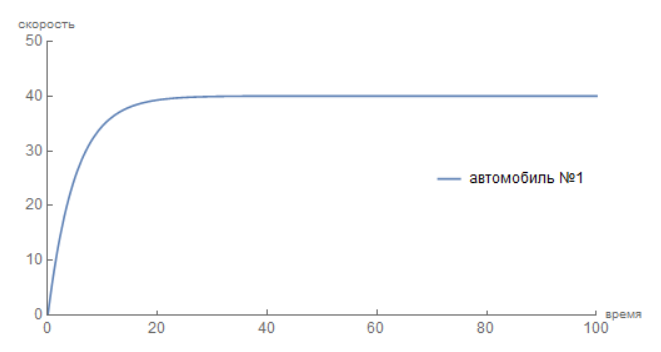
\includegraphics[width=1\linewidth,height=0.2\textheight]
			{Images/free_drive_speed.png}
		\end{minipage}
		\hfill 
		\begin{minipage}[h!]{0.48\linewidth}
			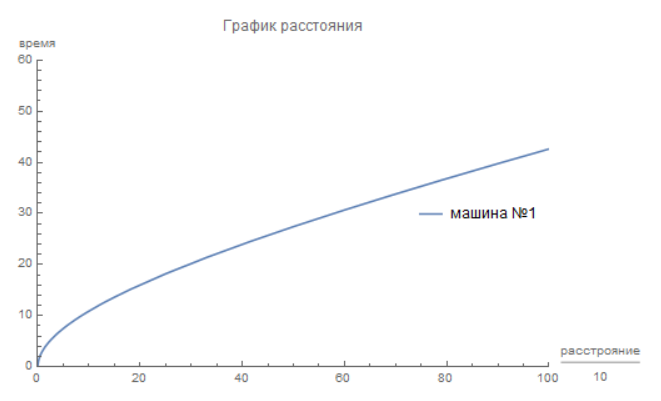
\includegraphics[width=1\linewidth,height=0.2\textheight]
			{Images/free_drive_distance.png}
		\end{minipage}
		\caption{Графики изменения скорости (слева) и расстояния (справа) для автомобиля при свободном движении без остановки с параметрами: $a=2$, $v_{max}=40$, $x_0=0$, $v_0=0$.}
		\label{free_drive_without_stop}
	\end{center}
\end{figure}

Как видно из графиков, автомобиль, разогнавшись до максимальной допустимой (желаемой) скорости, бесконечно двигается вперёд. Данная модель отлично описывает момент старта автомобиля, его разгон и движение с постоянной скоростью. В более жизненных ситуациях присутствуют процессы обратные разгону и старту - торможение и остановка.

Для описания остановки автомобиля рассмотрим следующее уравнение: 
\begin{equation} \label{stop_drive_with_initial_conditions}
\begin{cases}
\begin{split}
\ddot{x}(t) = \dfrac{1}{q}\left( v_{min} - \dot{x}(t)\right) \\
x(0)=x_0, \quad \dot{x}(0)=v_0
\end{split}
\end{cases}.
\end{equation}
Из уравнения \eqref{stop_drive_with_initial_conditions} видно, что остановка характеризуется минимальной (желаемой) скоростью $v_{min}$, начальной скоростью $v_{0}$, начальным положением транспортного средства $x_0$, коэффициентом торможения $q$. Под минимальной скоростью будем понимать ту скорость до которой водитель транспортного средства хочет снизить свою текущую скорость. Это не обязательно нулевая величина, в некоторых случаях водитель не хочет останавливаться полностью, а хочет лишь снизить скорость.

Уравнения \eqref{free_drive_with_initial_conditions} и  \eqref{stop_drive_with_initial_conditions} описывают два разных вида движения. Для того что бы получить полную модель свободного движения необходимо объединить полученные модели. Для этого введём две релейные функции $R_{a}(t)$ и $R_{b}(t)$.  

\begin{equation*} 
R_{a}(t)=
\begin{cases}
\begin{split}
&1, \quad t<t_{s} \\
&0, \quad t\geq t_{s}
\end{split}
\end{cases},
\qquad
R_{b}(t)=
\begin{cases}
\begin{split}
&0, \quad t<t_{s} \\
&1, \quad t\geq t_{s}
\end{split}
\end{cases}.
\end{equation*}

$R_{a}(t) = (1-R_{b}(t))$ и обозначим как $R(t)$

\begin{equation*} 
R(t)=
\begin{cases}
\begin{split}
&1, \quad t<t_{s} \\
&0, \quad t\geq t_{s}
\end{split}
\end{cases}.
\end{equation*}

\begin{equation} \label{free_drive_model}
\begin{cases}
\begin{split}
\ddot{x}(t) = &R(t) \left[ a\left( 1-\left( \dfrac{\dot{x}(t)}{v_{max}}\right) \right)\right] + (1-R(t))\left[  \dfrac{1}{q}\left( v_{min} - \dot{x}(t)\right) \right]  \\
&x(0)=x_0, \quad \dot{x}(0)=v_{0}
\end{split}
\end{cases}.
\end{equation}

\begin{table}[h!]
	\caption{Физическое значение параметров уравнения \eqref{free_drive_model}}
	\label{free_drive_parameters}
	\begin{center}
		\begin{tabularx}{\textwidth}{p{0.15\linewidth}p{0.85\linewidth}}			
			\hline
			\rule{0cm}{0,5cm}
			Параметр &  Физическое значение \\ 
			[3pt]\hline
			$a$ &\\
			$q$ &\\ 
			$v_{max}$ &\\
			$v_{min}$ &\\ 
			$x_0$ &\\
			$v_0$ &\\ 
			\hline
		\end{tabularx}
	\end{center}
\end{table}

\begin{figure}[h!]
	\begin{center}
		\begin{minipage}[h!]{0.48\linewidth}
			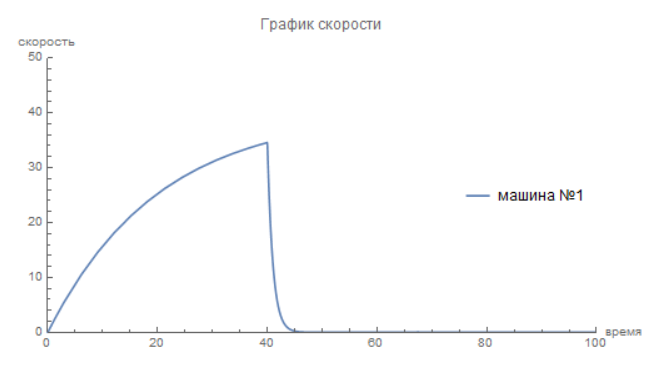
\includegraphics[width=1\linewidth,height=0.2\textheight]
			{Images/test12.png}
		\end{minipage}
		\hfill 
		\begin{minipage}[h!]{0.48\linewidth}
			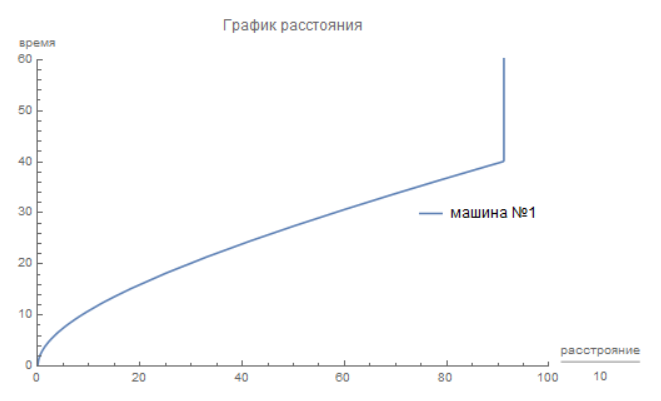
\includegraphics[width=1\linewidth,height=0.2\textheight]
			{Images/test22.png}
		\end{minipage}
		\caption{ПЕРЕДЕЛАТЬ}
		\label{free_drive_with_stop}
	\end{center}
\end{figure}

Полученная модель \eqref{free_drive_model} полностью описывает движение одного автомобиля на пустой дороге. 

\section{Модель следования за лидером}

Рассмотрим несколько автомобилей и занумеруем их индексом $n$ в соответствии с их порядковым номером на дороге. Предполагается, что ускорение $n$-ого автомобиля определяется состоянием соседних автомобилей, а именно наибольшее влияние оказывает непосредственно впереди идущий автомобиль (лидер).

Первая модель, основанная на принципе следования за лидером была разработана в 50-х годах прошлого века и предполагала, что каждый водитель адаптирует свою скорость к скорости лидирующего автомобиля:

\begin{equation} \label{follow_the_leader_first_model}
\ddot{x}_n(t) = \dfrac{1}{\gamma} (\dot{x}_{n-1}(t) - \dot{x}_{n}(t)), \\ 
\end{equation}
где $\gamma$ - время адаптации водителя.

Уравнение \eqref{follow_the_leader_first_model} было получено в работе  \cite{FirstFollowTheLeaderModel}. Эта модель является простой и плохо описывает свойства реального транспортного потока.

Произведём ряд модификаций модели \eqref{follow_the_leader_first_model}, которые позволят её улучшить. Введём в правую часть уравнения задержку аргумента по времени $\tau$, отражающую время реакции водителей на изменение скорости лидирующего автомобиля.  



\subsection{Модель следования за лидером без остановки}

Рассмотрим дифференциальное уравнение, которое описывает ускорение транспортного средства:

\begin{equation} \label{equation_for_acceleration}
\ddot{x}(t) = d (\dot{x}(t-\tau)-\dot{x}(t)),
\end{equation}
где $d$ - мощность двигателя, а $\tau$ - время реакции водителя.

Уравнение \eqref{equation_for_acceleration} зависит от скорости движения двух соседних автомобилей, то есть водитель автомобиля должен смотреть только на впереди идущий автомобиль. Конечно, в реальной жизни, водитель следит за движем большего количества транспортных средств, окружающих его, например, справа и слева, но при движении по прямой и без перестроений их влияние минимально.

Проинтегрировав уравнение \eqref{equation_for_acceleration} получаем следующее уравнение: 

\begin{equation} \label{equation_for_speed}
\dot{x}(t) = d(x(t-\tau) - x(t) - \lambda),
\end{equation}
где под $\lambda$ будем понимать безопасное расстояние между автомобилями.

Уравнение \eqref{equation_for_speed} служит для описания скорости транспортного средства и зависит от положения самого транспортного средства, положения впереди идущего транспортного средства и расстояния между ними. 

Дифференциальное уравнение \eqref{equation_for_speed} описывает лишь одно транспортное средство. Для описания всего потока запишем \eqref{equation_for_speed} в виде разностного уравнения:

\begin{equation} \label{difference_equation_for_speed}
\dot{x}_n(t) = d_n(x_{n-1}(t-\tau_n) - x_n(t) - \lambda_n).
\end{equation}

Без потери общности считаем, что все автомобили имеют одинаковые технические характеристики, а все водители одинаково оценивают дорожную ситуацию и реагируют на её изменения с одинаковой скоростью. Таким образом считаем, что $d_n = d$, $\tau_n = \tau$, $\lambda_n = \lambda$. Перепишем разностное уравнение \eqref{difference_equation_for_speed} в виде развёрнутой системы разностных уравнений:

\begin{equation} \label{equation_without_stopping}
\begin{cases}
\begin{split}
&\dot{x}_1(t) = d (v_{\max} t - x_1(t) - \lambda), \\ 
&\qquad x_1(0) = 0, \\
&\dot{x}_2(t) = d (x_1(t-\tau)-x_2(t) - \lambda), \\
&\qquad x_2(t) = -\lambda \quad t \in [-\tau, 0], \\
&\dot{x}_3(t) = d (x_2(t-\tau)-x_3(t) - \lambda), \\
&\qquad x_3(t) = -2\lambda \quad t \in [-2\tau, 0], \\
&\ldots \\
&\dot{x}_n(t) = d ({x}_{n-1}(t-\tau)-x_n(t) - \lambda), \\
&\qquad x_n(t) = -(n-1)\lambda \quad t \in [-(n-1)\tau, 0], \\
&\ldots \\
\end{split}
\end{cases}
\end{equation}

Обозначения, использующиеся в системе \eqref{equation_without_stopping}, приведены в таблице \ref{parameters}.

\begin{table}[h!]
	\caption{Физическое значение параметров уравнения \eqref{equation_without_stopping}}
	\label{parameters}
	\begin{center}
		\begin{tabularx}{\textwidth}{p{0.15\linewidth}p{0.85\linewidth}}			
			\hline
			\rule{0cm}{0,5cm}
			Параметр &  Физическое значение \\ 
			[3pt]\hline
			$n$ & порядковый номер автомобиля в потоке\\
			$d$ & мощность двигателя автомобиля \\
			$v_{max}$ & максимальная возможная (допустимая) скорость \\
			$\tau$ & время реакции водителя \\
			$\lambda $ & безопасное расстояние между автомобилями \\ 
			\hline
		\end{tabularx}
	\end{center}
\end{table}

Каждое отдельное уравнение системы \eqref{equation_without_stopping} соответствует автомобилю в потоке. На графиках (\ref{without_stop_d=0,122_tau=1}) и (\ref{without_stop_d=0,122_tau=5}) изображены графики длинны пути и скорости для нескольких автомобилей.

\begin{figure}[h!]
	\begin{center}
		\begin{minipage}[h!]{0.48\linewidth}
			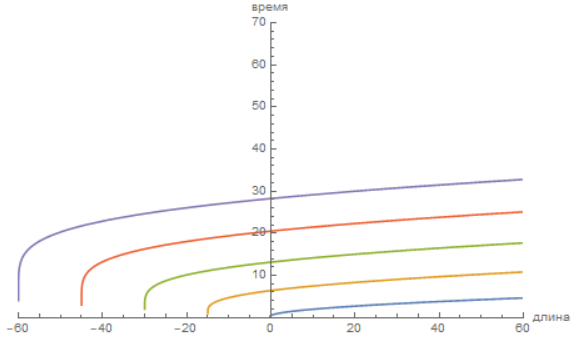
\includegraphics[width=1\linewidth,height=0.2\textheight]
			{Images/distance_without_stop_d=0,122_tau=1.png}
		\end{minipage}
		\hfill 
		\begin{minipage}[h!]{0.48\linewidth}
			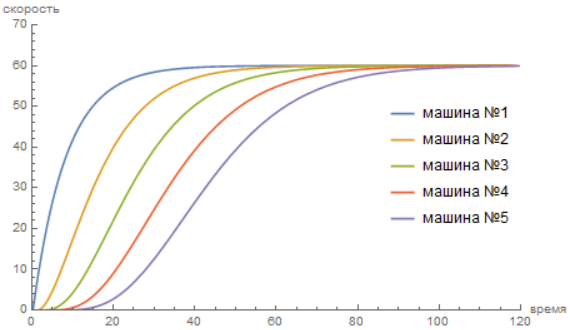
\includegraphics[width=1\linewidth,height=0.2\textheight]
			{Images/speed_without_stop_d=0,122_tau=1.png}
		\end{minipage}
		\caption{Графики изменения длин путей (слева) и скоростей (справа) для нескольких автомобилей при движении без остановки с параметрами: $\tau=1$, $\lambda=15$, $d=0,122$.}
		\label{without_stop_d=0,122_tau=1}
	\end{center}
\end{figure}

\begin{figure}[h!]
	\begin{center}
		\begin{minipage}[h!]{0.48\linewidth}
			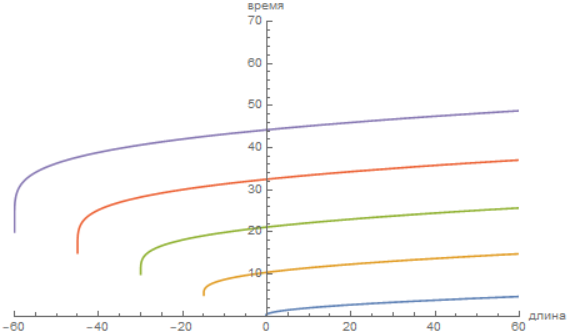
\includegraphics[width=1\linewidth,height=0.2\textheight]
			{Images/distance_without_stop_d=0,122_tau=5.png}
		\end{minipage}
		\hfill 
		\begin{minipage}[h!]{0.48\linewidth}
			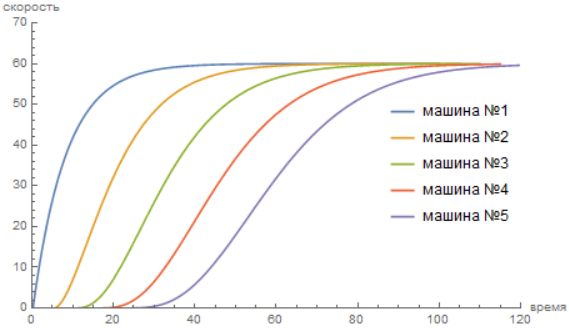
\includegraphics[width=1\linewidth,height=0.2\textheight]
			{Images/speed_without_stop_d=0,122_tau=5.png}
		\end{minipage}	
		\caption{Графики изменения длин путей (слева) и скоростей (справа) для нескольких автомобилей при движении без остановки с параметрами: $\tau=5$, $\lambda=15$, $d=0,122$.}
		\label{without_stop_d=0,122_tau=5}
	\end{center}
\end{figure}

Как видно из графиков, автомобили, разогнавшись до максимальной допустимой скорости, бесконечно едут на безопасном расстоянии друг от друга. Данная модель отлично подходит, если важен сам момент старта и разгон транспортных средств. В более жизненных ситуациях присутствуют процессы обратные разгону и движению - торможение и остановка. 

\subsection{Модель следования за лидером с остановкой}

Рассмотрим более реалистичную ситуацию, учитывающую торможение и остановку транспортного средства. Транспортные средства аналогично системе \eqref{equation_without_stopping} разгоняются и выходят на свою максимальную допустимую скорость, но через какое-то время им необходимо начать торможение и, в последствии, остановится. Так как все транспортные средства, кроме самого первого являются преследователями, то торможение стоит рассматривать лишь для первого, остальные сами отрегулируют свою скорость, относительно него. Математически это можно записать следующим образом:
  
\begin{equation} \label{stop_equation}
 S(t) = 
 \begin{cases}
 \begin{split}
 &v_{max} t \qquad &t \leqslant t_s \\
 &v_{max} t_s \qquad &t > t_s
 \end{split}
 \end{cases},
\end{equation}
где $t_s$ - время начала остановки.

Так как начало движения и набор скорости происходят аналогично предыдущему случаю, подставим  \eqref{stop_equation} в \eqref{equation_without_stopping} и получим модель движения транспортных средств с учётом начала торможения в момент времени $t_s$ и с последующей их остановкой. 
  
\begin{equation} \label{equation_with_stopping}
\begin{cases}
\begin{split}
&\dot{x}_1(t) = d (S(t) - x_1(t) - \lambda), \\ 
&\qquad x_1(0) = 0, \\
&\dot{x}_2(t) = d (x_1(t-\tau)-x_2(t) - \lambda), \\
&\qquad x_2(t) = -\lambda \quad t \in [-\tau, 0], \\
&\dot{x}_3(t) = d (x_2(t-\tau)-x_3(t) - \lambda), \\
&\qquad x_3(t) = -2\lambda \quad t \in [-2\tau, 0], \\
&\ldots \\
&\dot{x}_n(t) = d ({x}_{n-1}(t-\tau)-x_n(t) - \lambda), \\
&\qquad x_n(t) = -(n-1)\lambda \quad t \in [-(n-1)\tau, 0], \\
&\ldots \\
\end{split}
\end{cases}
\end{equation}

В модели \eqref{equation_with_stopping} скорость не зануляет полностью. Конечно, она близка к нулю, но всё же остаётся всегда положительной. При необходимости её можно занулить явно, когда она станет меньше какой-то наперёд заданной минимальной скорости транспортного средства, обусловленной техническими характеристиками. 
 
На графиках \eqref{with_stop_d=0,122_tau=1} изображены графики длинны пути и скорости для нескольких автомобилей. 
 \begin{figure}[h!]
 	\begin{center}
 		\begin{minipage}[h!]{0.48\linewidth}
 			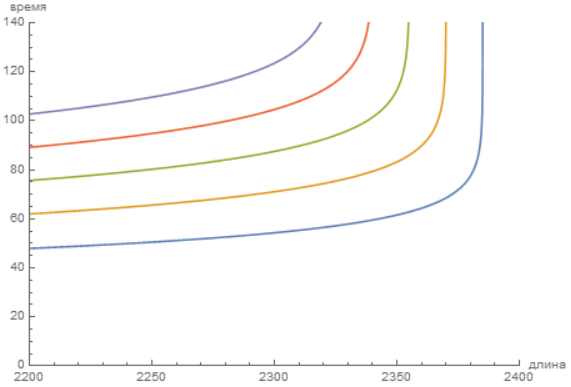
\includegraphics[width=1\linewidth,height=0.2\textheight]
 			{Images/distance_with_stop_d=0,122_tau=1.png}
 		\end{minipage}
 		\hfill 
 		\begin{minipage}[h!]{0.48\linewidth}
 			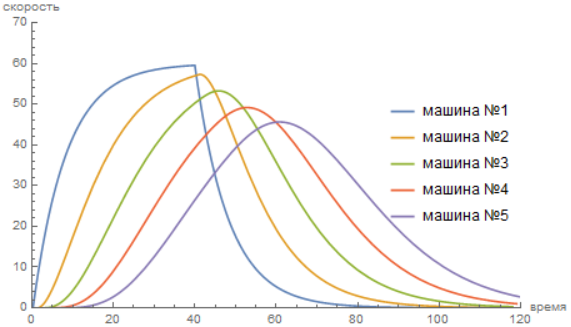
\includegraphics[width=1\linewidth,height=0.2\textheight]
 			{Images/speed_with_stop_d=0,122_tau=1.png}
 		\end{minipage}
 		\caption{Графики изменения длин путей (слева) и скоростей (справа) для нескольких автомобилей при движении с остановкой с параметрами: $\tau=1$, $\lambda=15$, $d=0,122$.}
 		\label{with_stop_d=0,122_tau=1}
 	\end{center}
 \end{figure}

Как видно из графиков, автомобили, в определённой момент времени $t_s$, начинают тормозить и останавливаются на безопасном расстоянии друг от друга. 

Данная модель отлично подходит, если важен не только момент старта и разгон, но так же торможение и остановка.

\section{Модель Газиса}

\begin{equation} \label{gazis_model}
\ddot{x}_n(t) = \dfrac{\lambda_{l,m}\dot{x}_n^m(t)}{(x_{n-1}(t-\tau)-x_n(t-\tau))^l}(\dot{x}_{n-1}(t-\tau)-\dot{x}_{n}(t))
\end{equation}

\begin{table}[h!]
	\caption{Физическое значение параметров уравнения \eqref{gazis_model}}
	\label{gazis_parameters}
	\begin{center}
		\begin{tabularx}{\textwidth}{p{0.15\linewidth}p{0.85\linewidth}}			
			\hline
			\rule{0cm}{0,5cm}
			Параметр &  Физическое значение \\ 
			[3pt]\hline
			$\tau$ & время реакции водителя \\
			$m, l$ & параметры скорости и расстояния движения \\
			$\lambda_{l,m} $ & константа, характеризующая движение  \\ 
			\hline
		\end{tabularx}
	\end{center}
\end{table} 

\section{Практическое применение} 

Состояние дел в области моделирования транспортных потоков на сегодняшний день таково, что, не смотря на значительный прогресс, полное понимание природы автомобильных проблем ещё не достигнуто. Учёные
говорят, что они пока находятся ближе к пониманию процессов зарождения Вселенной, чем, например, образования автомобильных заторов. 

Российское законодательство предусматривает ГОСТ для организации дорожного движения \cite{Gost}.Но данный ГОСТ не охватывает множество дорожных проблем, например, такую важную проблему как светофорное регулирование, в частности время горения сигналов на светофоре. Пункт 7.4. "Режимы работы светофоров"  данного ГОСТа описывает внешний вид светофора, последовательность сигналов и другое, но время горения каждого сигнала регулируется для каждого светофора и перекрёстка самостоятельно дорожными службами на местах. Такое регулирование приводит к множеству проблем, ведь можно не всегда удачно отрегулировать режим работы светофора с первого раза, и это может привести к серьёзным последствиям, таким как пробки и заторы, а в некоторых случаях даже спровоцировать дорожно транспортные прошествия.

В большинстве случаев настройка светофоров производится экспериментальным путём. Такие экспериментальные 
работы по оптимизации светофорного регулирования привели к настоящему транспортному коллапсу в Ярославле.
Утром 28 февраля 2018 года на Московском проспекте, проспекте Фрунзе, Суздальском шоссе и других прилегающих к улицах машины встали в огромную пробку, около пяти километров. Произошло несколько аварий \cite{News}. Такие ситуации не редкость, из чего следует, что технологии управления дорожным движением надо менять на более современные, например, на математическое моделирование движения транспортных потоков, которое можно исследовать использования компьютерные технологии. 

Модели \eqref{equation_without_stopping} и \eqref{equation_with_stopping} отлично подходят для моделирования начала движения транспорта со светофора на перекрёстках. С их помощью можно определить оптимальное время и оптимальную проходимость транспорта через светофор. 

Модели можно интерпретировать как реальную ситуацию, в которой в начальный момент времени, все автомобили стоят на безопасном расстоянии друг от друга перед светофором, на котором горит красный свет (рис. \ref{car's_start_position}). Затем на светофоре загорается зелёный свет и все автомобили начинают движение. Если дальнейшая судьба, уехавших машин не важна, то можно использовать \eqref{equation_without_stopping}. В противном же случае  \eqref{equation_with_stopping}.

\begin{figure}[h!]  
	\begin{center}
		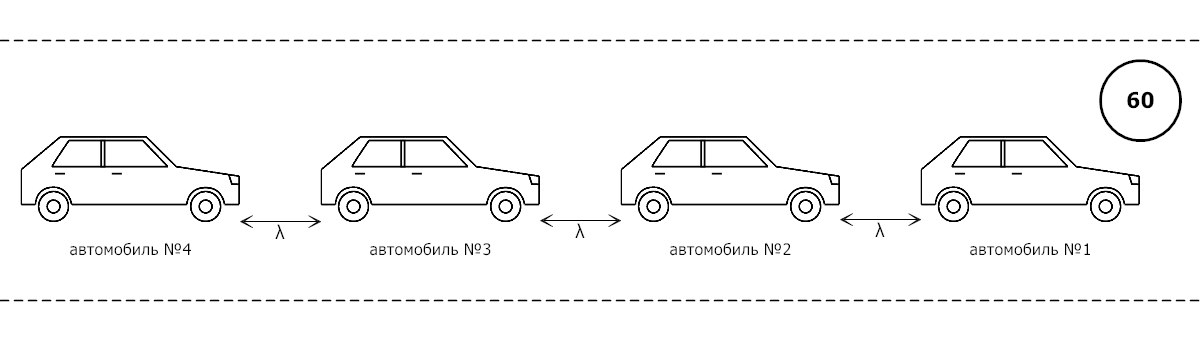
\includegraphics[keepaspectratio,width=160mm,height=70mm]{Images/car's_start_position.png}
	\end{center}
	\caption{Автомобили в момент старта.}
	\label{car's_start_position}
\end{figure}

Наибольшее влияние на проходимость транспортных средств через светофор оказываю мощность транспортного средства $d$ и время реакции водителя $\tau$, поэтому для различных значений этих параметров для системы \eqref{equation_without_stopping}. составлена таблица \eqref{table_without_stopping}. В этой таблице приведено количество транспортных средств, которые пройдут через светофор за время $t=40$ и будут соблюдать безопасную дистанцию $\lambda = 150$.  
 
\begin{table}[h!]
	\caption{Количество транспортных средств для модели \eqref{equation_without_stopping}}
	\label{table_without_stopping}
	\begin{center}
		\begin{tabular}{|l|*{5}{c|}}\hline
			\backslashbox{$d$}{$\tau$}
			&\makebox[3em]{1}&\makebox[3em]{2}&\makebox[3em]{3}	&\makebox[3em]{4}&\makebox[3em]{5}
			\\\hline
			0.1 &3&3&3&3&2
			\\\hline
			0.5 &7&6&5&5&4
			\\\hline
			1 &9&7&6&6&5
			\\\hline
			2 &10&8&7&6&5
			\\\hline
			3 &11&9&7&6&5
			\\\hline
		\end{tabular}
	\end{center}
\end{table} 

В таблице \eqref{table_with_stopping} приведено количество транспортных средств для системы \eqref{equation_with_stopping}, в которой время $t=40$ безопасная дистанция $\lambda = 150$, а время начала остановки $t_s=20$. 

\begin{table}[h!]
	\caption{Количество транспортных средств для модели \eqref{equation_with_stopping}}
	\label{table_with_stopping}
	\begin{center}
		\begin{tabular}{|l|*{5}{c|}}\hline
			\backslashbox{$d$}{$\tau$}
			&\makebox[3em]{1}&\makebox[3em]{2}&\makebox[3em]{3}	&\makebox[3em]{4}&\makebox[3em]{5}
			\\\hline
			0.1 &3&2&2&2&1
			\\\hline
			0.5 &7&5&5&3&2
			\\\hline
			1 &9&6&5&4&2
			\\\hline
			2 &10&7&6&5&3
			\\\hline
			3 &11&10&7&6&4
			\\\hline
		\end{tabular}
	\end{center}
\end{table} 
 
В таблицах \eqref{table_without_stopping} и \eqref{table_with_stopping} приведены данные для каких-то значений, немеющих ничего общего с реальными данными, но и из них отчётливо видно, что проходимость транспортного потока различна при различных параметрах и может быть оптимизирована. Изучение реальных параметров и подстановка их в модели \eqref{equation_without_stopping} и \eqref{equation_with_stopping} даст точный результат, позволит смоделировать реальную жизненную ситуацию и поможет оптимизировать технологии управления транспортными потоками.

\vspace{\baselineskip} \vspace{\baselineskip} \vspace{\baselineskip} 
\vspace{\baselineskip} \vspace{\baselineskip} \vspace{\baselineskip}
\hspace{0pt}

\newpage
\section*{Заключение}
\addcontentsline{toc}{section}{Заключение}
На основе проведённых исследований можно сделать вывод, что теоретический подход, основанный на принципе следования транспортных средств друг за другом, позволяет построить содержательную математическую модель для описания движения транспортных потоков. С использованием этого теоретического подхода было построено две математические модели  \eqref{equation_without_stopping} и \eqref{equation_with_stopping}, которые имеют большую прикладную значимость. На основе этих моделей можно исследовать различные жизненные ситуации, например, смоделировать начало движения автомобилей, найти оптимальную проходимость транспортных средств через светофор и множество других аналогичных ситуаций. Все исследования можно проводить с использованием компьютерных технологий, что позволит сделать технологии управления дорожным движением более современными.

\newpage

\begin{thebibliography}{**}
	\bibitem{Street}
	Дубелиръ Г.Д. "Городскiя улицы и мостовыя". 1912.
	\bibitem{TrafficFlow}
	https://spravochnick.ru/logistika/logisticheskie\_potoki/transportnyy\_potok/
	\bibitem{GippsModel}
	Wilson R. E. Gipps’ Model of Highway Traffic. 2002.
	\bibitem{FirstFollowTheLeaderModel}
	Pipes L.A. An operational analysis of traffic
 dynamics. 1953. 
%	\bibitem{Polygon}
%	Выгодский М.Я. Справочник по элементарной математике. 2001.
% 	\bibitem{Runge_Kutta}
%	 Бахвалов Н.С.  Численные методы. 1975.  
%	\bibitem{Refactoring}
%	Мартин Ф. Рефакторинг. Улучшение существующего кода. 2008.
	\bibitem{Gost}
	"ГОСТ Р 52289-2004. Национальный стандарт Российской Федерации. Технические средства организации дорожного движения. Правила применения дорожных знаков, разметки, светофоров, дорожных ограждений и направляющих устройств" (утв. Приказом Ростехрегулирования от 15.12.2004 N 120-ст) (ред. от 09.12.2013)
	\bibitem{News}
	https://www.yar.kp.ru/daily/26801.4/3835277/
\end{thebibliography}

\end{document}